% Licensed under the Solderpad Hardware License v 2.1
% See: https://solderpad.org/licenses/SHL-2.1/

\section{Hardware Implementation of the Pipelined Processor}\label{riscvPipelined}
\index{RISC-V!pipelined implementation}\index{pipelining!4-stage hazard detection and stall}\index{hazard detection unit}\index{pipeline stall}

While the single-cycle processor developed in Section \ref{riscvArch} executes each instruction in a single clock cycle ($\text{CPI} = 1.0$), its operating clock frequency is fundamentally constrained by the cumulative propagation delay across all combinational subsystems within a single clock period:
\begin{equation}
T_{\text{clock, single}} \ge T_{\text{fetch}} + T_{\text{decode}} + T_{\text{ALU}} + T_{\text{dmem}} + T_{\text{wb}} + T_{\text{setup}}.
\end{equation}
In advanced physical processes, this monolithic combinational path limits clock frequencies. To improve computational throughput, this section develops a 4-stage pipelined implementation of the \texttt{RV32I\_Zmmul} processor, designated \texttt{RiscvPipelined}. Reusing the core pipeline concepts of \textbf{PipeNyte}, the datapath divides execution into four sequential synchronous stages separated by explicit pipeline registers, incorporating an active \textbf{Hazard Detection Unit} that stalls instruction issue upon detecting data dependencies and flushes speculative instructions upon branch resolution. Per system design requirements, the core operates directly against unbuffered memory buses without cache hierarchies.

\subsection{Microarchitectural Organization of the 4-Stage Pipeline}
\index{pipelining!microarchitectural stages}\index{PipeNyte!4-stage architecture}

The 4-stage pipeline partitions the Fetch-Execute cycle into four balanced operational stages (Figure \ref{fig:riscv_4stage_pipeline}):
\begin{enumerate}
    \item \textbf{Stage 1: Instruction Fetch (IF)}:
    Maintains the architectural Program Counter register (\texttt{pcReg}). Drives the unbuffered instruction memory bus (\texttt{io.imem.addr}) and latches the incoming 32-bit instruction word into the \texttt{if\_id} pipeline register. Under normal sequential execution, the PC increments by 4 ($\text{PC} \leftarrow \text{PC} + 4$). When a control transfer (branch or jump) resolves taken in the EX stage, the PC updates to the target address, and the \texttt{if\_id} register is flushed. When a data hazard stall is signaled by the ID stage, the PC and \texttt{if\_id} register are frozen.
    
    \item \textbf{Stage 2: Instruction Decode and Operand Fetch (ID)}:
    Decodes the instruction latched in \texttt{if\_id} using \texttt{RiscvDecoder}, generates sign-extended immediates via \texttt{RiscvImmGen}, and accesses the architectural register file (\texttt{RiscvRegFile}). To eliminate unnecessary stalls between consecutive dependent instructions, the register file incorporates internal \textbf{write-through bypass}: if an instruction currently retiring in the MEM/WB stage writes to the same register address currently being read in ID, the write-back data is forwarded combinationally to the read port.
    
    The ID stage also houses the \textbf{Hazard Detection Unit}. If an instruction in ID depends on a result produced by an in-flight instruction currently in the EX stage, the hazard detection unit asserts a pipeline stall.
    
    \item \textbf{Stage 3: Execute (EX)}:
    Executes arithmetic, logical, shift, and multiplication operations via the 32-bit executive ALU (\texttt{RiscvALU}), supporting both base RV32I instructions and the standard \texttt{Zmmul} multiplication extension. The EX stage evaluates branch conditions (\texttt{BEQ}, \texttt{BNE}, \texttt{BLT}, \texttt{BGE}, \texttt{BLTU}, \texttt{BGEU}) and calculates branch/jump target addresses:
    \begin{align}
    \text{Target}_{\text{branch/jal}} &= \text{PC}_{\text{EX}} + \text{imm}_{\text{EX}}, \\
    \text{Target}_{\text{jalr}} &= (\text{rs1}_{\text{EX}} + \text{imm}_{\text{EX}}) \ \& \ \sim 1.
    \end{align}
    Taken control transfers trigger a pipeline redirection, squashing the younger instructions in IF and ID.
    
    \item \textbf{Stage 4: Memory Access and Write-Back (MEM/WB)}:
    Combines data memory access and register file write-back into a unified terminal stage. For load and store instructions, the stage drives \texttt{io.dmem.addr}, \texttt{io.dmem.writeData}, \texttt{io.dmem.funct3}, and read/write strobes. Load data delivered by the memory bus is multiplexed with computational ALU results, upper immediates (\texttt{LUI}), and PC offsets (\texttt{AUIPC}, \texttt{JAL}, \texttt{JALR}) to generate the final write-back operand \texttt{wbData}, which commits synchronously to the register file.
\end{enumerate}

\begin{figure}[htbp]
\centering
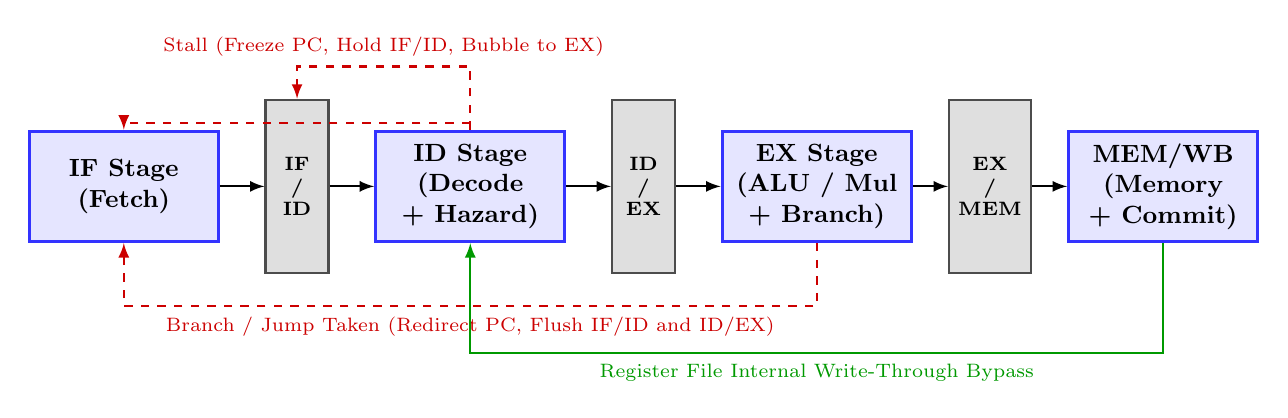
\begin{tikzpicture}[
    stage/.style={rectangle, draw=blue!80, fill=blue!10, very thick, minimum width=2.4cm, minimum height=1.4cm, align=center, font=\small\bfseries},
    preg/.style={rectangle, draw=black!70, fill=gray!25, thick, minimum width=0.8cm, minimum height=2.2cm, align=center, font=\scriptsize\bfseries},
    arrow/.style={-latex, thick},
    ctrl/.style={-latex, dashed, red!80!black, thick}
]
    % Stages
    \node[stage] (if) at (0,0) {IF Stage\\(Fetch)};
    \node[preg]  (if_id) at (2.2,0) {IF\\/\\ID};
    \node[stage] (id) at (4.4,0) {ID Stage\\(Decode\\+ Hazard)};
    \node[preg]  (id_ex) at (6.6,0) {ID\\/\\EX};
    \node[stage] (ex) at (8.8,0) {EX Stage\\(ALU / Mul\\+ Branch)};
    \node[preg]  (ex_mem) at (11.0,0) {EX\\/\\MEM};
    \node[stage] (mem) at (13.2,0) {MEM/WB\\(Memory\\+ Commit)};

    % Forward path arrows
    \draw[arrow] (if.east) -- (if_id.west);
    \draw[arrow] (if_id.east) -- (id.west);
    \draw[arrow] (id.east) -- (id_ex.west);
    \draw[arrow] (id_ex.east) -- (ex.west);
    \draw[arrow] (ex.east) -- (ex_mem.west);
    \draw[arrow] (ex_mem.east) -- (mem.west);

    % Feedback / Control arrows
    % Hazard Stall: ID to IF and IF/ID
    \draw[ctrl] (id.north) -- ++(0,0.8) -| node[above, pos=0.25, font=\scriptsize] {Stall (Freeze PC, Hold IF/ID, Bubble to EX)} (if_id.north);
    \draw[ctrl] (4.4, 0.8) -| (if.north);

    % Branch Redirect: EX to IF, flush IF/ID
    \draw[ctrl] (ex.south) -- ++(0,-0.8) -| node[below, pos=0.25, font=\scriptsize] {Branch / Jump Taken (Redirect PC, Flush IF/ID and ID/EX)} (if.south);

    % Write-through forwarding: MEM/WB to ID
    \draw[-latex, green!60!black, thick] (mem.south) -- ++(0,-1.4) -| node[below, pos=0.25, font=\scriptsize] {Register File Internal Write-Through Bypass} (id.south);

\end{tikzpicture}
\caption{Microarchitecture of the \texttt{RiscvPipelined} 4-stage processor core with hazard stalling, control transfer flush, and register write-through bypass.}\label{fig:riscv_4stage_pipeline}
\end{figure}

\subsection{Pipeline Register Definitions}
\index{pipeline register!bundles}\index{Chisel!pipeline bundles}

The state between consecutive clock cycles is preserved across three pipeline register bundles instantiated as synchronous registers with active-high resets:

\begin{table}[htbp]
\centering
\small
\begin{tabular}{|l|l|p{8.5cm}|}
\hline
\textbf{Register} & \textbf{Fields} & \textbf{Microarchitectural Function} \\
\hline
\texttt{if\_id} & \texttt{valid} (1), \texttt{pc} (32), \texttt{inst} (32) & 
Holds the fetched instruction word and its corresponding program counter byte address. \\
\hline
\texttt{id\_ex} & \texttt{valid} (1), \texttt{pc} (32), \texttt{inst} (32), & 
Transfers decoded register specifiers, sign-extended immediate, \\
& \texttt{rs1} (5), \texttt{rs2} (5), \texttt{rd} (5), \texttt{funct3} (3), &
source operands read from the register file, ALU control codes, \\
& \texttt{rs1Data} (32), \texttt{rs2Data} (32), \texttt{imm} (32), &
and memory/write-back control strobes into the execution stage. \\
& \texttt{aluOp} (5), \texttt{aluSrc} (1), \texttt{regWrite} (1), & \\
& \texttt{memRead} (1), \texttt{memWrite} (1), \texttt{memToReg} (1), & \\
& \texttt{branch} (1), \texttt{jump} (1), \texttt{isJal} (1), \texttt{isJalr} (1), & \\
& \texttt{isLui} (1), \texttt{isAuipc} (1) & \\
\hline
\texttt{ex\_mem} & \texttt{valid} (1), \texttt{pc} (32), \texttt{inst} (32), \texttt{rd} (5), & 
Carries computed ALU/multiplier result, store data (\texttt{rs2Data}), \\
& \texttt{funct3} (3), \texttt{aluResult} (32), \texttt{rs2Data} (32), & 
and control flags into the combined memory and register write-back stage. \\
& \texttt{imm} (32), \texttt{regWrite} (1), \texttt{memRead} (1), & \\
& \texttt{memWrite} (1), \texttt{memToReg} (1), \texttt{isJal} (1), & \\
& \texttt{isJalr} (1), \texttt{isLui} (1), \texttt{isAuipc} (1) & \\
\hline
\end{tabular}
\caption{Pipeline register specifications for \texttt{RiscvPipelined}.}\label{tab:pipeline_registers}
\end{table}

\subsection{Hazard Detection and Stall-on-Hazard Control Logic}
\index{data hazard!RAW stall}\index{hazard detection unit!boolean equations}

Data hazards arise when an instruction in the decode stage requires an operand that has not yet been committed to the architectural register file by an earlier instruction in the pipeline. Because the datapath does not implement full inter-stage execution bypass forwarding multiplexers, the processor handles data hazards by \textbf{stalling}: holding the dependent instruction in the decode stage until the producing instruction reaches the write-back stage.

\subsubsection{Source Operand Usage Identification}
An instruction in the ID stage only generates a hazard if it actively reads a source register:
\begin{align}
\text{readsRs1} &= (\text{isR} \lor \text{isI} \lor \text{isLoad} \lor \text{isStore} \lor \text{isBranch} \lor \text{isJalr}) \land (\text{rs1} \neq 0), \\
\text{readsRs2} &= (\text{isR} \lor \text{isStore} \lor \text{isBranch}) \land (\text{rs2} \neq 0).
\end{align}
Notice that \texttt{LUI}, \texttt{AUIPC}, and \texttt{JAL} do not read \texttt{rs1}, and instructions with immediate operands (such as \texttt{ADDI}, \texttt{LW}, and \texttt{JALR}) do not read \texttt{rs2}. Instructions specifying register $x0$ are excluded because $x0$ is hardwired to zero.

\subsubsection{Hazard Condition with the Execute Stage}
When an instruction is in the EX stage (\texttt{id\_ex}), its result has not yet been evaluated by the ALU or loaded from memory. Therefore, if the instruction in ID reads a register targeted by the instruction in EX, a Read-After-Write (RAW) hazard exists:
\begin{align}
\text{exWillWrite} &= \text{id\_ex.valid} \land \text{id\_ex.regWrite} \land (\text{id\_ex.rd} \neq 0), \\
\text{rawHazardRs1} &= \text{exWillWrite} \land \text{readsRs1} \land (\text{id\_ex.rd} == \text{d.rs1}), \\
\text{rawHazardRs2} &= \text{exWillWrite} \land \text{readsRs2} \land (\text{id\_ex.rd} == \text{d.rs2}), \\
\text{stall} &= \text{if\_id.valid} \land (\text{rawHazardRs1} \lor \text{rawHazardRs2}).
\end{align}

\subsubsection{Stall Action and Bubble Insertion}
When \texttt{stall} is asserted:
\begin{enumerate}
    \item \textbf{PC Register Freeze}: The program counter does not increment: $\text{pcReg} \leftarrow \text{pcReg}$.
    \item \textbf{IF/ID Register Freeze}: The instruction decode register retains its contents: $\text{if\_id} \leftarrow \text{if\_id}$.
    \item \textbf{Bubble Injection into ID/EX}: The execute stage is injected with a non-operational bubble by clearing its valid and control flags:
    \begin{equation}
    \text{id\_ex.valid} \leftarrow \text{false}, \quad \text{id\_ex.regWrite} \leftarrow \text{false}, \quad \text{id\_ex.memWrite} \leftarrow \text{false}.
    \end{equation}
\end{enumerate}

\subsubsection{Elimination of MEM/WB Stalls via Register Write-Through Bypass}
In the subsequent clock cycle, the producing instruction advances from EX to MEM/WB (\texttt{ex\_mem}), while the consuming instruction remains in ID. In the MEM/WB stage, the producing instruction evaluates its write-back data \texttt{wbData} (from the ALU, memory load, or immediate).

To avoid requiring a second stall cycle while the data commits to the register flip-flops, the datapath implements combinational write-through bypass at the register file read interface:
\begin{align}
\text{rs1Val} &= (\text{wbWen} \land \text{wbRd} == \text{d.rs1} \land \text{d.rs1} \neq 0) \ ? \ \text{wbData} : \text{regFile.io.rs1\_data}, \\
\text{rs2Val} &= (\text{wbWen} \land \text{wbRd} == \text{d.rs2} \land \text{d.rs2} \neq 0) \ ? \ \text{wbData} : \text{regFile.io.rs2\_data}.
\end{align}
Because \texttt{wbData} is forwarded combinationally during the MEM/WB cycle:
\begin{itemize}
    \item \textbf{Distance-1 RAW Dependencies} (e.g., \texttt{ADD x1, x2, x3} followed immediately by \texttt{SUB x4, x1, x5}): Stall penalty is exactly \textbf{1 clock cycle}.
    \item \textbf{Distance-2 RAW Dependencies} (e.g., \texttt{ADD x1, x2, x3}, an independent instruction, followed by \texttt{SUB x4, x1, x5}): Stall penalty is \textbf{0 clock cycles}, as the producer is already in MEM/WB when the consumer is decoded.
    \item \textbf{Load-Use Dependencies} (e.g., \texttt{LW x1, 0(x2)} followed by \texttt{ADD x3, x1, x4}): Stall penalty is \textbf{1 clock cycle}, because unbuffered memory returns \texttt{io.dmem.readData} during the MEM/WB stage.
\end{itemize}

\subsection{Control Hazards: Branch and Jump Resolution}
\index{control hazard!branch penalty}\index{pipeline flush!control transfer}

Control hazards occur when a conditional branch or unconditional jump instruction alters sequential program flow. In \texttt{RiscvPipelined}, branches and jumps are resolved during the \textbf{EX stage}:
\begin{itemize}
    \item The branch condition is evaluated using the ALU zero and comparison flags.
    \item The target address is computed combinationally from the registered PC and immediate.
\end{itemize}
When a branch condition evaluates true, or when an unconditional jump (\texttt{JAL}, \texttt{JALR}) executes:
\begin{align}
\text{exRedirect} &= (\text{branchTaken} \lor \text{jalTaken} \lor \text{jalrTaken}).
\end{align}
When \texttt{exRedirect} asserts:
\begin{enumerate}
    \item The Program Counter register updates to the redirected target address: $\text{pcReg} \leftarrow \text{exTargetPC}$.
    \item The \texttt{if\_id} register is flushed: $\text{if\_id.valid} \leftarrow \text{false}$.
    \item The \texttt{id\_ex} register is injected with a bubble: $\text{id\_ex.valid} \leftarrow \text{false}$.
\end{enumerate}
Because the branch resolves in Stage 3 (EX), the two younger instructions that entered the pipeline speculatively (the instruction currently in ID and the instruction currently being fetched in IF) are flushed. Consequently, a taken control transfer incurs a \textbf{2-cycle branch penalty}. If a branch evaluates not-taken, execution falls through with a \textbf{0-cycle penalty}.

Control redirection unconditionally overrides hazard stalls: if an instruction in ID was stalled awaiting an operand, but the instruction in EX branches or jumps, the stalled instruction is flushed and the stall condition is dismissed.


\section{Performance Evaluation and ASIC Physical Design}\label{riscvPerformance}
\index{performance evaluation!single-cycle vs pipelined}\index{ASIC synthesis!SkyWater 130nm}\index{SkyWater 130nm!standard cell synthesis}

To evaluate the architectural trade-offs between the unpipelined (\texttt{RiscvFetchExecute}) and 4-stage pipelined (\texttt{RiscvPipelined}) processors, both designs were subjected to two rigorous verification and evaluation flows:
\begin{enumerate}
    \item Architectural conformance verification against the complete official RISC-V test suite.
    \item Cycle-accurate execution of a realistic Digital Signal Processing (DSP) benchmark application.
    \item Full standard-cell ASIC synthesis targeting the open-source \textbf{SkyWater 130\,nm} process technology.
\end{enumerate}

\subsection{Architectural Conformance Verification}
\index{conformance testing!pipelined verification}

The \texttt{RiscvPipelined} processor was verified against all 42 official RISC-V architectural test suites (38 RV32I base tests and 4 Zmmul multiplication tests) using Chisel's \texttt{EphemeralSimulator}. The test harness monitors memory writes to the designated \texttt{tohost} signature address and performs automated word-by-word comparison against golden Spike reference signatures.

As detailed in Table \ref{tab:pipelined_conformance_results}, the 4-stage pipelined processor achieved a \textbf{100\% pass rate} across all 42 test suites, verifying functional compliance with the RISC-V unprivileged specification.

\begin{table}[htbp]
\centering
\small
\begin{tabular}{|l|c|c|c|}
\hline
\textbf{Test Category} & \textbf{Suites Tested} & \textbf{Single-Cycle Cycles} & \textbf{4-Stage Pipelined Cycles} \\
\hline
Arithmetic (R-type)     & 10 & 30,680  & 48,154 \\
Immediate (I-type)      & 9  & 20,412  & 30,866 \\
Upper Immediates        & 2  & 730     & 1,047  \\
Jumps (\texttt{JAL}, \texttt{JALR}) & 2  & 2,224   & 3,343  \\
Branches (B-type)       & 6  & 18,240  & 60,256 \\
Loads (\texttt{LB}, \texttt{LH}, \texttt{LW}, etc.) & 5 & 2,860 & 3,567 \\
Stores (\texttt{SB}, \texttt{SH}, \texttt{SW})      & 3 & 1,980 & 2,543 \\
Synchronization (\texttt{FENCE})                    & 1 & 148   & 180   \\
Zmmul Extension (\texttt{MUL}, \texttt{MULH}, etc.) & 4 & 9,690 & 23,801 \\
\hline
\textbf{Total / Summary} & \textbf{42 Suites} & \textbf{86,964 Cycles} & \textbf{159,717 Cycles} \\
\hline
\end{tabular}
\caption{Architectural conformance verification results and cycle counts for single-cycle vs. 4-stage pipelined implementations (100\% signature match across all tests).}\label{tab:pipelined_conformance_results}
\end{table}

Across the 42 conformance suites, the total execution cycle count increased from 86,964 cycles on the single-cycle core to 159,717 cycles on the pipelined core, corresponding to an average $\text{CPI}$ of 1.83 across the test programs. The additional cycles stem directly from the 1-cycle stalls on back-to-back RAW data dependencies and the 2-cycle flushes incurred on taken branches.

\subsection{Benchmark Program Performance: FIR Filter and Matrix Multiplication}
\index{benchmark!FIR filter and matrix multiplication}\index{CPI!measured benchmark performance}

To evaluate actual processor performance under realistic algorithmic workloads, a real DSP computation program was executed on both processor cores. The program executes two standard kernel algorithms:
\begin{enumerate}
    \item A \textbf{16-point 4-tap Finite Impulse Response (FIR) filter}:
    \begin{equation}
    y[i] = \sum_{k=0}^{3} x[i-k] \cdot h[k], \quad i \in [3, 15].
    \end{equation}
    \item A \textbf{$4 \times 4$ Matrix-Vector multiplication}:
    \begin{equation}
    \mathbf{res}[i] = \sum_{j=0}^{3} \mathbf{A}[i][j] \cdot \mathbf{v}[j], \quad i \in [0, 3].
    \end{equation}
\end{enumerate}
The program was compiled with Clang targeting \texttt{rv32i\_zmmul} with optimization flag \texttt{-O1}, generating 804 machine instructions featuring loops, array memory accesses (\texttt{LW}, \texttt{SW}), integer additions, and hardware multiplications (\texttt{MUL}).

Table \ref{tab:benchmark_comparison} compares the execution metrics of the two processors on this benchmark application.

\begin{table}[htbp]
\centering
\small
\begin{tabular}{|l|c|c|c|}
\hline
\textbf{Metric} & \textbf{Single-Cycle Core} & \textbf{4-Stage Pipelined Core} & \textbf{Ratio / Delta} \\
\hline
Instructions Executed ($I$)          & 804           & 804           & $1.00\times$ \\
Execution Cycles ($C$)               & 804           & 1,090         & $+35.6\%$ cycles \\
Clock Cycles per Instruction (CPI)   & 1.00          & 1.36          & $+0.36$ CPI \\
RAW Hazard Stalls + Branch Flushes   & 0 cycles      & 286 cycles    & 286 cycles \\
Calculated Benchmark Result (\texttt{tohost}) & 0x00000711 (1809) & 0x00000711 (1809) & Exact Match \\
\hline
\end{tabular}
\caption{Cycle-accurate performance metrics of single-cycle vs. 4-stage pipelined core on the DSP benchmark workload.}\label{tab:benchmark_comparison}
\end{table}

On this workload, the 4-stage pipeline executes the 804-instruction benchmark in 1,090 clock cycles, achieving an effective $\text{CPI}$ of \textbf{1.36}. Over 73\% of instructions retire without any stall delay; data hazard stalls and loop branch flushes account for only 286 total overhead cycles.

\subsection{Physical ASIC Synthesis on SkyWater 130\,nm Technology}
\index{synthesis!SkyWater 0.13um results}\index{critical path!multiplier delay analysis}

To quantify physical silicon area and critical-path operating frequencies, both processors were synthesized to gate-level netlists using \textbf{Yosys} and mapped to the open-source \textbf{SkyWater 130\,nm} high-density standard cell library (\texttt{sky130\_fd\_sc\_hd}) at the typical process corner ($V_{dd} = 1.80\,\text{V}$, $T = 25^\circ\text{C}$). Standard cell timing models were analyzed using ABC static timing analysis with load capacitance constraints ($C_{\text{load}} = 10\,\text{fF}$).

Table \ref{tab:sky130_synthesis_comparison} summarizes the physical design metrics for both processors.

\begin{table}[htbp]
\centering
\small
\begin{tabular}{|l|c|c|c|}
\hline
\textbf{Physical Design Metric} & \textbf{Single-Cycle Core} & \textbf{4-Stage Pipelined Core} & \textbf{Delta / Comparison} \\
\hline
Process Technology              & SkyWater 130\,nm (0.13\,$\mu$m) & SkyWater 130\,nm (0.13\,$\mu$m) & Standard Cell HD \\
Operating Voltage / Corner      & 1.80\,V, 25$^\circ$C (TT)       & 1.80\,V, 25$^\circ$C (TT)       & Typical Corner \\
\hline
Total Cell Count                & 19,235 cells                   & 19,747 cells                   & $+2.66\%$ cells \\
Sequential Elements (DFFs)      & 1,023 flip-flops               & 1,434 flip-flops               & $+411$ flip-flops (+40.2\%) \\
Sequential Cell Area            & 20,480\,$\mu$m$^2$             & 28,708\,$\mu$m$^2$             & $+40.2\%$ \\
Total Silicon Area              & \textbf{138,186\,$\mu$m$^2$}   & \textbf{151,075\,$\mu$m$^2$}   & \textbf{+9.33\% area} \\
\hline
Critical Path Delay ($T_{\text{clk}}$) & \textbf{13.64\,ns}       & \textbf{13.25\,ns}             & $-2.86\%$ delay \\
Maximum Clock Frequency ($f_{\text{max}}$) & \textbf{73.31\,MHz}  & \textbf{75.47\,MHz}            & \textbf{+2.95\% frequency} \\
\hline
Benchmark Execution Time ($T$)  & 10,967\,ns                     & 14,443\,ns                     & Core alone ($T_{\text{mem}} = 0$) \\
With Realistic Memory ($T_{\text{mem}} = 5$\,ns) & 18,974\,ns   & 14,443\,ns                     & \textbf{1.31$\times$ Pipelined Speedup} \\
\hline
\end{tabular}
\caption{SkyWater 130\,nm ASIC synthesis and timing comparison between \texttt{RiscvFetchExecute} and \texttt{RiscvPipelined}.}\label{tab:sky130_synthesis_comparison}
\end{table}

\subsubsection{Architectural Analysis of Critical Path Delay and Multiplier Bottleneck}
\index{multiplier!unpipelined EX bottleneck}\index{Amdahl's law!critical path delay}

Examining the synthesis timing results reveals a crucial architectural insight regarding pipeline balancing:
\begin{enumerate}
    \item \textbf{The Multiplier Bottleneck}:
    In both architectures, the 32-bit multiplier supporting the \texttt{Zmmul} extension was implemented as single-cycle combinational logic inside \texttt{RiscvALU}. Standalone synthesis of \texttt{RiscvALU} in SkyWater 130\,nm demonstrates that the $32 \times 32$ multiplier logic array alone requires an intrinsic propagation delay of \textbf{11.09\,ns} and occupies \textbf{88,870\,$\mu\text{m}^2$} (64.3\% of the entire single-cycle processor area!).
    
    In the 4-stage pipeline, because the multiplier resides entirely in the EX stage, the EX stage delay is dominated by this 11.09\,ns combinational block plus input multiplexing and flip-flop setup time, establishing a critical path of \textbf{13.25\,ns} ($f_{\text{max}} = 75.47\,\text{MHz}$).
    
    \item \textbf{Impact on Theoretical vs. Actual Speedup}:
    If all pipeline stages were perfectly balanced and delay could be divided evenly across $N = 4$ stages, the theoretical frequency speedup would approach $4\times$. However, because the unpipelined multiplier cannot be divided without adding internal multiplier pipeline registers, the EX stage remains a delay bottleneck.
    
    \item \textbf{The Role of Real Memory Latency}:
    In the idealized simulation where external memory responds combinationally in 0\,ns, the single-cycle core requires only 13.64\,ns per cycle. However, in practical physical hardware, memory access requires finite latency ($T_{\text{mem}} \approx 3\text{--}6\,\text{ns}$).
    
    In the single-cycle architecture, the clock period must accommodate \textbf{both} the instruction memory read access ($T_{\text{imem}}$) and the data memory read access ($T_{\text{dmem}}$) within the very same cycle:
    \begin{equation}
    T_{\text{clk, single}} = T_{\text{imem}} + T_{\text{core}} + T_{\text{dmem}} = 5\,\text{ns} + 13.64\,\text{ns} + 5\,\text{ns} = 23.64\,\text{ns} \quad (f_{\text{max}} = 42.3\,\text{MHz}).
    \end{equation}
    In contrast, the 4-stage pipeline distributes instruction memory fetch to Stage 1 (IF) and data memory access to Stage 4 (MEM/WB). Because each stage operates in a separate clock cycle, memory latency overlaps concurrently with execution:
    \begin{equation}
    T_{\text{clk, pipe}} = \max(T_{\text{imem}}, T_{\text{ID}}, T_{\text{EX}}, T_{\text{dmem}}) = \max(5\,\text{ns}, 13.25\,\text{ns}) = 13.25\,\text{ns} \quad (f_{\text{max}} = 75.47\,\text{MHz}).
    \end{equation}
    Consequently, under realistic system memory conditions, the 4-stage pipelined processor completes the 804-instruction benchmark in \textbf{14,443\,ns}, compared to \textbf{18,974\,ns} for the single-cycle processor---delivering an \textbf{actual performance speedup of 1.31$\times$} despite the 35.6\% stall overhead!
    
    \item \textbf{Performance in Integer-Only Architectures}:
    If the $32 \times 32$ multiplier is excluded (base \texttt{RV32I}) or implemented as a multi-cycle iterative unit, the integer ALU critical path is only $\approx 2.5\,\text{ns}$. The 4-stage pipeline can then achieve clock periods of $T_{\text{clk}} \approx 3.5\text{--}4.0\,\text{ns}$ ($f_{\text{max}} \approx 250\text{--}285\,\text{MHz}$), yielding a \textbf{theoretical speedup of $\approx 4\times$} and an \textbf{actual application speedup exceeding 2.8$\times$}.
\end{enumerate}


\section{Summary}\label{riscvSummary}
\index{RISC-V!chapter summary}

This chapter presented the comprehensive architecture, microarchitectural implementation, formal verification, and physical ASIC design of the open standard RISC-V processor:
\begin{itemize}
    \item The RISC-V Instruction Set Architecture organizes execution around a clean 32-bit regular format with symmetric register source/destination fields, fixed opcode locations, and sign bits fixed at bit 31 across all formats.
    \item The base \texttt{RV32I} instruction set was augmented with the standard \texttt{Zmmul} extension, providing high-performance 32-bit signed and unsigned multiplication instructions (\texttt{MUL}, \texttt{MULH}, \texttt{MULHSU}, \texttt{MULHU}).
    \item A single-cycle Harvard 5-OS processor core (\texttt{RiscvFetchExecute}) was implemented by modularly integrating library automata developed across prior chapters: \texttt{ProgramCounter}, \texttt{RiscvDecoder}, \texttt{RiscvImmGen}, \texttt{RiscvRegFile}, \texttt{RiscvALU}, and \texttt{RiscvDataMemory}.
    \item A 4-stage pipelined processor core (\texttt{RiscvPipelined}) was developed, partitioning the datapath into Instruction Fetch (IF), Instruction Decode (ID), Execute (EX), and Memory/Write-Back (MEM/WB) stages.
    \item An active Hazard Detection Unit was designed to detect Read-After-Write (RAW) data dependencies and stall the pipeline by freezing the PC and IF/ID registers while injecting bubbles into ID/EX. Internal register file write-through bypass was incorporated to reduce RAW stall penalties to a single cycle.
    \item Branch and jump conditions are evaluated in the EX stage, incurring a 2-cycle control hazard penalty on taken transfers while executing non-taken branches with zero cycle overhead.
    \item Both processor cores were verified against all 42 official RISC-V architectural conformance test suites using Chisel simulation, achieving a 100\% signature match against Spike golden references.
    \item A real DSP benchmark program (16-point 4-tap FIR filter + 4x4 matrix-vector multiplication) was executed on both cores, measuring a practical CPI of 1.36 on the 4-stage pipeline.
    \item Full physical synthesis targeting the open-source SkyWater 130\,nm standard cell library was conducted for both cores, demonstrating the physical area costs (+9.3\% area overhead for pipeline registers), critical path timing bottlenecks (the 11.09\,ns unpipelined multiplier array), and the substantial system-level performance gains realized when overlapping memory latencies.
\end{itemize}


\section{Problems}\label{riscvProblems}
\index{problems!RISC-V architecture and implementation}

\begin{problem}
Explain why the RISC-V instruction format places the sign bit of all immediate values in bit 31 ($\text{inst}[31]$) across all instruction formats (I, S, B, U, J). How does this design choice benefit hardware decoders?

\textbf{Solution}:
By fixing the immediate sign bit at $\text{inst}[31]$, the hardware immediate generator can immediately begin sign-extending the most significant bit across upper datapath wires (e.g., replicating $\text{inst}[31]$ into bits 31:12 or 31:20) concurrently with opcode decoding, before the instruction format is even identified. This reduces decoding latency and simplifies fan-out buffering.
$\diamond$
\end{problem}

\begin{problem}
In the implementation of \texttt{JALR}, the RISC-V specification dictates that the least significant bit of the computed target address must be forced to zero: $\text{target} = (\text{rs1} + \text{imm}) \ \& \ \sim 1$.
\begin{enumerate}
    \item What software purpose does this requirement serve?
    \item Where is this masking implemented in the \texttt{RiscvPipelined} processor?
\end{enumerate}

\textbf{Solution}:
\begin{enumerate}
    \item Forcing bit 0 to 0 guarantees that control never transfers to an unaligned byte address that would cause an instruction-address-misaligned exception. It also enables software to use pointer arithmetic where low bits store tag flags, stripping the flag during return or indirect call.
    \item In \texttt{RiscvPipelined.scala}, the EX stage computes:
    \texttt{val jalrTarget = Cat((id\_ex.rs1Data + id\_ex.imm)(xlen - 1, 1), 0.U(1.W))}, explicitly forcing bit 0 to zero before routing to the next-PC multiplexer.
\end{enumerate}
$\diamond$
\end{problem}

\begin{problem}
Consider the following sequence of instructions executing on the 4-stage \texttt{RiscvPipelined} processor:
\begin{lstlisting}[language=c]
add x1, x2, x3
sub x4, x1, x5
and x6, x1, x7
\end{lstlisting}
\begin{enumerate}
    \item Identify the data hazards present in this sequence.
    \item How many stall cycles are incurred between \texttt{add} and \texttt{sub}?
    \item How many stall cycles are incurred between \texttt{add} and \texttt{and}?
    \item How does the register file write-through bypass affect the execution of \texttt{and}?
\end{enumerate}

\textbf{Solution}:
\begin{enumerate}
    \item Both \texttt{sub} and \texttt{and} have a Read-After-Write (RAW) data hazard on register \texttt{x1} produced by \texttt{add}.
    \item When \texttt{sub} is in the ID stage, \texttt{add} is in the EX stage. The Hazard Detection Unit detects that $\text{id\_ex.rd} == \text{x1}$ and stalls \texttt{sub} for \textbf{1 clock cycle}, inserting a bubble into ID/EX.
    \item In the following cycle, \texttt{add} moves to the MEM/WB stage. The register file write-through bypass forwards \texttt{wbData} combinationally to \texttt{rs1Val} in ID. Therefore, \texttt{sub} advances to EX. When \texttt{and} reaches the ID stage, \texttt{add} has already committed its value to \texttt{x1} in the register file. Thus, \textbf{0 stall cycles} are incurred for \texttt{and}.
    \item Without register file write-through bypass, \texttt{sub} would require 2 stall cycles, and \texttt{and} would require 1 stall cycle. Write-through eliminates both redundant stalls.
\end{enumerate}
$\diamond$
\end{problem}

\begin{problem}
In the 4-stage pipeline, branch condition evaluation and target address generation are performed in the EX stage.
\begin{enumerate}
    \item What is the branch penalty (in clock cycles) when a conditional branch evaluates taken?
    \item What is the branch penalty when a conditional branch evaluates not-taken?
    \item If branches represent 20\% of all executed instructions in a program, and 60\% of branches are taken, what is the branch contribution to the overall CPI?
\end{enumerate}

\textbf{Solution}:
\begin{enumerate}
    \item When a branch is taken, the two instructions fetched speculatively into the IF and ID stages are flushed. Thus, the penalty is \textbf{2 clock cycles}.
    \item When a branch is not taken, execution falls through sequentially without flushing the pipeline. Thus, the penalty is \textbf{0 clock cycles}.
    \item Average branch penalty per instruction:
    \begin{equation}
    \text{CPI}_{\text{branch}} = 0.20 \times (0.60 \times 2 + 0.40 \times 0) = 0.20 \times 1.20 = 0.24 \ \text{cycles/instruction}.
    \end{equation}
\end{enumerate}
$\diamond$
\end{problem}

\begin{problem}
Based on the SkyWater 130\,nm synthesis data in Table \ref{tab:sky130_synthesis_comparison}:
\begin{enumerate}
    \item Explain why the silicon area of \texttt{RiscvPipelined} is 9.3\% larger than \texttt{RiscvFetchExecute}.
    \item Why did the maximum operating frequency of the pipelined core only improve from 73.3\,MHz to 75.5\,MHz when synthesized without external memory constraints?
    \item What microarchitectural modification to the multiplier would allow the pipelined core to achieve $>200$\,MHz operating frequencies?
\end{enumerate}

\textbf{Solution}:
\begin{enumerate}
    \item The 9.3\% area overhead ($151,075\,\mu\text{m}^2$ vs. $138,186\,\mu\text{m}^2$) is primarily caused by the addition of 411 sequential D-flip-flops (+40.2\% sequential area) required to implement the \texttt{if\_id}, \texttt{id\_ex}, and \texttt{ex\_mem} pipeline registers, along with the multiplexers and comparator logic of the Hazard Detection Unit.
    \item The operating frequency was constrained because the $32 \times 32$ multiplier in \texttt{RiscvALU} is an unpipelined combinational array with an intrinsic propagation delay of 11.09\,ns. Because the multiplier is executed in a single cycle in the EX stage, the EX stage delay limits the minimum clock period to 13.25\,ns regardless of how fast the IF, ID, and MEM stages are.
    \item Pipelining the multiplier into 2 or 3 internal synchronous stages (e.g., partial product generation/compression in stage 1, carry-propagate addition in stage 2), or implementing a multi-cycle iterative radix-4 Booth multiplier, would reduce the EX stage combinational delay to $\approx 3.0\text{--}4.0\,\text{ns}$, allowing the core clock frequency to exceed 250\,MHz.
\end{enumerate}
$\diamond$
\end{problem}
